\subsection{bottom\_bc}%
%

% - Purpose & Problem description:
%     These first two parts give reader short details about the test case,
%     the physical phenomena involved and specify how the numerical solution will be validated
%
\subsubsection{Purpose}
%
This test case is used to validate the boundary conditions on the bed fo Telemac-3D simulations
%
\subsubsection{Description of the problem}
%
In this test case two simulations will be run. In \texttt{t3d\_bottom\_inlet.f} a flow rate will be imposed using the boundary conditions on the bed, whereas in \texttt{t3d\_bottom\_source.cas} a source discharge will imposed on a node on the bed as a source term.


%% - Reference:
%%     This part gives the reference solution we are comparing to and
%%     explicits the analytical solution when available;
%%
%%
%\subsubsection{Reference}
%%
%
%% - Physical parameters:
%%     This part specifies the geometry, details all the physical parameters
%%     used to describe both porous media (soil model in particularly) and
%%     solute characteristics (dispersion/diffusion coefficients, soil <=> pollutant interactions...)
%%
%%
%\subsubsection{Physical parameters}
%%

% - Geometry and Mesh:
%     This part describes the mesh used in the computation
%
%
\subsubsection{Geometry and Mesh}
%
The configuration of this test case is simple, it is a square box of sides $4000$ m. The depth is constant, and initially set to $500$ m. The geometry of the test case is shown in figure \ref{fig:GeomPlan}.

\begin{figure}[t!]
\begin{center}
	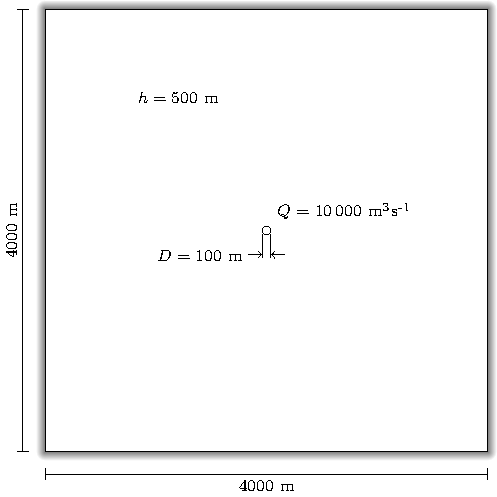
\includegraphics[]{./GeomPlan.pdf}
\end{center}
\caption{Geometrical parameters of the test case.}
\label{fig:GeomPlan}
\end{figure}

Furthermore, two different meshes will be used, a fine mesh and a coarse mesh. Since source terms are imposed on a node, the coarse mesh is used to impose the inflow on a single node, and it will be used for \texttt{t3d\_bottom\_source.cas}. Since applying a flow rate can be done on several nodes on the bed, the finer mesh will be compared to the coarse mesh for \texttt{t3d\_bottom\_inlet.cas} simulation results. The coarseness of the mesh is also present for the distribution of the planes in the simulation. The fine mesh has a smaller plane spacing near the bed and the free surface, whereas the coarse mesh has the same number of planes, but these are distributed evenly on the bottom half of the domain and the plane spacing decreases towards the free-surface.

% - Initial and boundary conditions:
%     This part details both initial and boundary conditions used to simulate the case
%
%
\subsubsection{Initial and Boundary Conditions}
%
A discharge $Q$ of $10\,000$ m\textsuperscript{3}s\textsuperscript{-1} will be imposed inside a circle with diameter $D$ of $100$ meters placed at the centre of the bed. All vertical boundaries will be defined as walls, see figure \ref{fig:GeomPlan}.


% - Numerical parameters:
%     This part is used to specify the numerical parameters used
%     (adaptive time step, mass-lumping when necessary...)
%
%
\subsubsection{Numerical parameters}
%
The key numerical parameters for \texttt{t3d\_bottom\_inlet.f} are:

\begin{itemize}
\item \texttt{OPEN BOUNDARY CONDITIONS ON THE BED = YES}
\item \texttt{PRESCRIBED FLOWRATES ON THE BED = 10000.}
\item \texttt{NON-HYDROSTATIC VERSION : YES}
\end{itemize}

The key numerical parameters for \texttt{t3d\_bottom\_source.cas} are:

\begin{itemize}
\item \texttt{ABSCISSAE OF SOURCES = 2000.0}
\item \texttt{ORDINATES OF SOURCES = 2000.0}
\item \texttt{ELEVATIONS OF SOURCES = -500.0}
\item \texttt{WATER DISCHARGE OF SOURCES = 10000}
\item \texttt{NON-HYDROSTATIC VERSION : YES}
\end{itemize}

% - Results:
%     We comment in this part the numerical results against the reference ones,
%     giving understanding keys and making assumptions when necessary.
%
%
\subsubsection{Results}
%
At the moment, no post processing is done, however it would be good to have a comparison of the water depth profiles at $y=2000$ m and the vertical velocity profiles at $x=2000$ m and $y=2000$ m. Contour plots of the vertical velocities at $y=2000$ m would also be useful.

% Here is an example of how to include the graph generated by validateTELEMAC.py
% They should be in test_case/img
%\begin{figure} [!h]
%\centering
%\includegraphics[scale=0.3]{../img/mygraph.png}
% \caption{mycaption}\label{mylabel}
%\end{figure}


